\documentclass[uplatex,dvipdfmx, 10pt, aspectratio=43]{beamer}
\usepackage{graphicx}
\usepackage{amsmath}
\usepackage{latexsym}
\usepackage{multirow}
\usepackage{url}
\usepackage[separate-uncertainty]{siunitx}
\usepackage{physics}
\usepackage{enumerate}
\usepackage{bm}
\usepackage{pdfpages}
\usepackage{pxchfon}
\usepackage{tikz}
\usepackage{float}
\usepackage{listings}
\usepackage{amsfonts}
\usepackage{empheq}

% tikz pakcage
\usepackage{tikz}

% theories package
\usepackage{amsmath}
\usepackage{amsthm}

% algorithm package
\usepackage{algorithm}
\usepackage{algorithmic}

\usetheme[block=fill]{metropolis}

% blcok layout
\setbeamertemplate{blocks}[rounded][shadow=true]

% title
\title{情報工学工房最終発表}
\author{2311081 木村 慎之介}
\institute{電気通信大学 情報理工学域 Ⅰ類 コンピュータサイエンスプログラム 3年}
\date{\today}

% insert index at top of each section
\AtBeginSection{
    \begin{frame}{目次}
        \tableofcontents[currentsection]
    \end{frame}
}

% navigation var
\setbeamertemplate{some beamer element}{square}

\begin{document}
\frame{\maketitle}

% index
\begin{frame}{目次}
    \tableofcontents
\end{frame}

\section{テーマについて}
\begin{frame}{テーマについて}
    \begin{block}{組み合わせゲーム}
        次の2つの性質を満たすゲームを組み合わせゲームという。
        \begin{itemize}
            \item さいころを振るなどといったランダムな要素を含まない(確定性)
            \item 山札や手牌といった盤面に表示されない情報がない(完全情報性)
        \end{itemize}
    \end{block}
    例えばチェスや将棋は組み合わせゲームではあるが、麻雀やすごろくなどは該当しない。\cite{combinatorial_game_theory}
\end{frame}

\begin{frame}{テーマについて}
    \begin{block}{Chomp(チョコレートゲーム)}
        \begin{columns}[totalwidth=\linewidth]
            \begin{column}{.55\linewidth}
                以下の手順に沿って進めていくゲームをChompという。
                \begin{itemize}
                    \item チョコレートのマスのうち1つを選んで、そのマスを含む右下の領域を食べる(消す)
                    \item お互いに順番にチョコレートを食べていって、最後に一番左上の毒のチョコレートを食べたら負け
                \end{itemize}
            \end{column}
            \begin{column}{.49\linewidth}
                \centering
                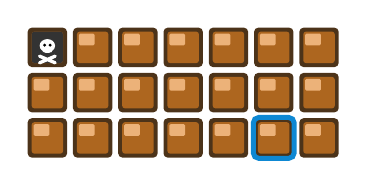
\begin{tikzpicture}[scale=0.5]
                    % チョコレートのマスを描画
                    \foreach \x in {0,...,6} {
                        \foreach \y in {0,...,2} {
                            % 外枠（暗い茶色）
                            \fill[brown!40!black, rounded corners=1.5pt]
                                (\x*1.15, -\y*1.15) rectangle ++(1.0, -1.0);
                            % 内側（明るい茶色）
                            \fill[brown!60!orange!80!black, rounded corners=1pt]
                                (\x*1.15+0.1, -\y*1.15-0.1) rectangle ++(0.8, -0.8);
                            % ハイライト（上面の光沢）
                            \fill[brown!50!orange!60!white, rounded corners=0.5pt]
                                (\x*1.15+0.15, -\y*1.15-0.15) rectangle ++(0.4, -0.3);
                        }
                    }
                    % 毒マス（左上）— 黒背景にドクロ
                    \fill[black!80, rounded corners=1pt]
                        (0.1, -0.1) rectangle ++(0.8, -0.8);
                    % ドクロ（TikZで描画）
                    \begin{scope}[shift={(0.5, -0.5)}, scale=0.28, white]
                        % 頭
                        \fill (0, 0.15) circle [x radius=0.7, y radius=0.6];
                        % 顎
                        \fill[rounded corners=1pt] (-0.4, -0.2) rectangle (0.4, -0.5);
                        % 目
                        \fill[black] (-0.25, 0.2) circle (0.15);
                        \fill[black] (0.25, 0.2) circle (0.15);
                        % 骨（クロス）
                        \draw[white, line width=1.2pt, line cap=round]
                            (-0.7, -0.8) -- (0.7, -1.4)
                            (0.7, -0.8) -- (-0.7, -1.4);
                        % 骨の端（丸）
                        \foreach \p in {(-0.7,-0.8),(0.7,-0.8),(-0.7,-1.4),(0.7,-1.4)} {
                            \fill[white] \p circle (0.12);
                        }
                    \end{scope}
                    % 選択マス（青枠）— 3行目6列目
                    \draw[cyan!70!blue, line width=1.8pt, rounded corners=2pt]
                        (5*1.15-0.02, -2*1.15+0.02) rectangle ++(1.04, -1.04);
                \end{tikzpicture}
            \end{column}
        \end{columns}
    \end{block}
\end{frame}

\begin{frame}{テーマについて}
    今回はChompというゲームを題材に「各プレイヤーがランダムに手を打つようなことを考えたら、どのような数学的特徴が見えるだろうか」という問いを立てて活動を行った。
\end{frame}

\section{先行研究}
\begin{frame}{先行研究}
    先行研究\cite{ramdom_combinatorial_game_theory}ではプレイヤーがランダムに手を進めるような状況をモデル化し、そのモデル化における一部の初期盤面に対する先手の勝率が解析された。
\end{frame}

\begin{frame}{先行研究}
    \begin{block}{モデル化}
        各プレイヤーは、与えられた盤面から一様ランダムにマスを選択する。
        このとき、盤面\(B\)における先手の勝率\(P(B)\)は以下のように再帰的に求まる。
        \begin{equation}
            P(B) = 1 - \frac{1}{|B|} \sum_{B \rightarrow C} P(C)
        \end{equation}
        ここで\(B \rightarrow C\)とは、盤面\(C\)は盤面\(B\)から1手で遷移されることを、\(|B|\)は盤面\(B\)のマスの数を表す。
    \end{block}
\end{frame}

\begin{frame}{先行研究}
    \begin{block}{盤面が1行の場合の先手の勝率}
        盤面が1行の場合、先手の勝率\(P(B)\)は次のように求まる。
        \begin{equation}
            P(B) = \left\{
                \begin{aligned}
                    & 1 \ (|B| = 0) \\
                    & 0 \ (|B| = 1) \\
                    & \frac{1}{2} \ (|B| \geq 2)
                \end{aligned}
            \right.
        \end{equation}
    \end{block}
\end{frame}

\begin{frame}{先行研究}
    \begin{block}{盤面が2行の場合の先手の勝率}
        盤面が2行の場合、上から1行目のマスの数を\(n\)、2行目のマスの数を\(k \ (k \leq n)\)としたとき、先手の勝率は以下のように再帰的に求めることができる。
        \begin{equation}
            P(n, k) = \frac{1}{2} - \frac{n \alpha_k + \beta_k}{\left(2\left(k - 1\right)\right)! \cdot \left(n + k\right)\left(n + k - 1\right)\left(n + k - 2\right)}
        \end{equation}
        ただし、\(\alpha_k, \beta_k\)は初期値を\(\alpha_1 = 1, \beta_1 = -1\)とする次の漸化式で表される。
        \begin{align}
            & \alpha_{k + 1} = \left(4k^2 + k\right)\alpha_k + \beta_k \\
            & \beta_{k + 1} = -k\left(k + 1\right)\alpha_k + \left(4k^2 -k -1\right)\beta_k
        \end{align}
    \end{block}
\end{frame}

\section{課題の設定と結果}
\begin{frame}{課題の設定と結果}
    先行研究の結果を利用して先手の勝率を可視化して観察した。
    また、観察結果からみられた特徴を数学的に証明することを試みた。
\end{frame}

\begin{frame}{課題の設定と結果}
    先手の勝率の可視化は次の2つの方法に分けて行った。
    \begin{itemize}
        \item ランダムに手を打つプレイヤーのシミュレーションをプログラムで組んで、その時の先手の勝率を可視化
        \item 3行の盤面に固定して、モデル化で提示した再帰式から計算して、その結果をグラフに可視化
    \end{itemize}
\end{frame}

\begin{frame}{課題の設定と結果}
    \begin{figure}
        \centering
        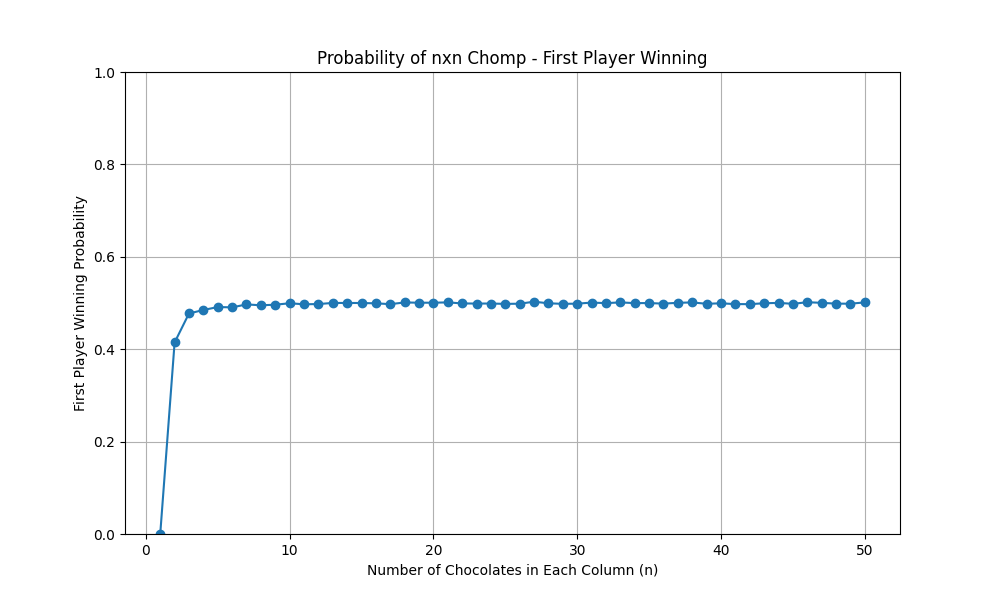
\includegraphics[width=0.6\columnwidth]{research/figures/visualize_simulated_prob.png}
        \caption{シミュレーションの可視化}
    \end{figure}
\end{frame}

\begin{frame}{課題の設定と結果}
    \begin{figure}
        \centering
        \begin{minipage}[b]{0.49\columnwidth}
            \centering
            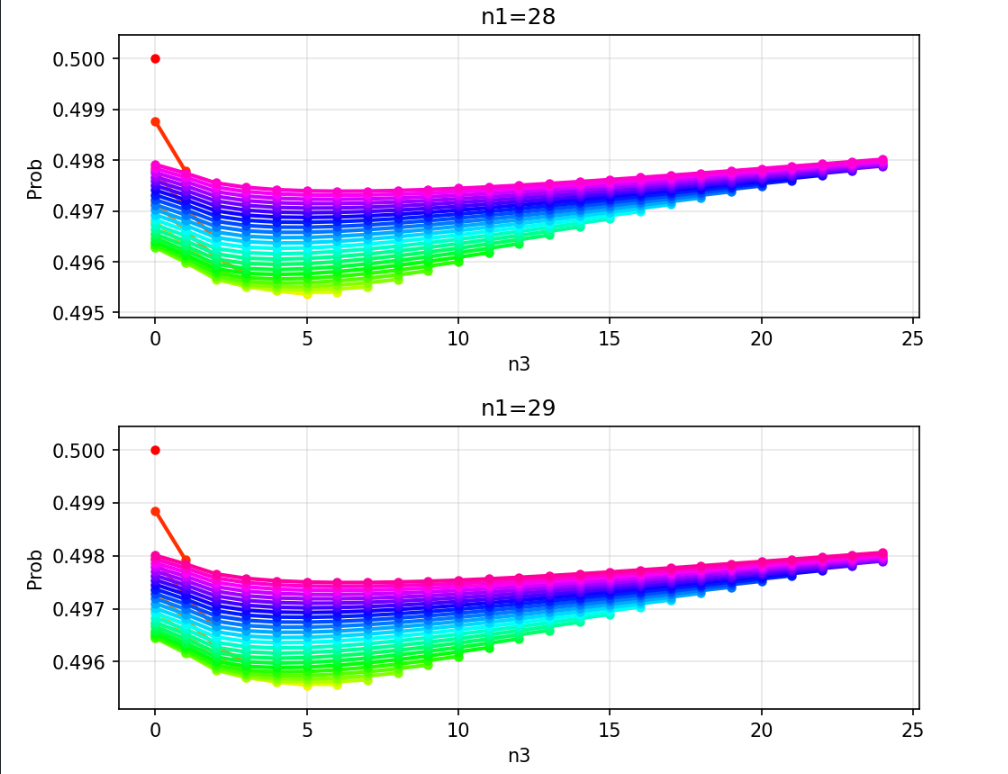
\includegraphics[width=0.9\columnwidth]{research/figures/visualize_prob_overlap_row.png}
        \end{minipage}
        \begin{minipage}[b]{0.49\columnwidth}
            \centering
            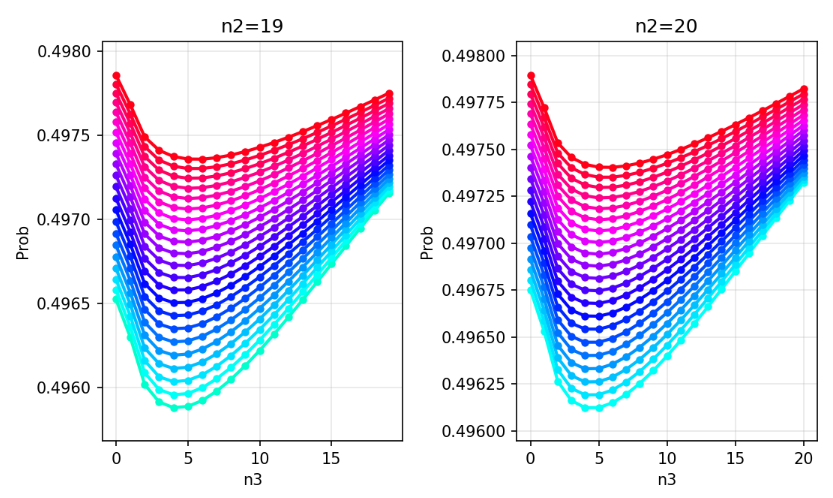
\includegraphics[width=0.9\columnwidth]{research/figures/visualize_prob_overlap_col.png}
        \end{minipage}
        \caption{3行に固定された盤面における先手の勝率の可視化}
    \end{figure}
\end{frame}

\begin{frame}{課題の設定と結果}
    可視化から、以下のことを考えた。
    \begin{itemize}
        \item ある一定のところを超えると確率が単調に増加する
        \item 勝率は(見える範囲では)\(0.5\)を下回っている
    \end{itemize}
\end{frame}

\begin{frame}{課題の設定と結果}
    \begin{block}{盤面の包含関係と確率の単調性についての予想}
        盤面\(B\)と\(B'\)について、2つの盤面の間に\(|B| = |B'| + 1\)という関係があり、かつ\(|B|\)が十分に大きいとき
        \begin{equation}
            P(B) \geq P(B')
        \end{equation}
        という関係がある
    \end{block}
\end{frame}

\begin{frame}{課題の設定とその結果}
    \begin{block}{盤面の包含関係と確率の大小関係についての予想}
        \begin{align}
            P(B) - P(B')    &= \left(1 - \frac{1}{|B|} \sum_{B \rightarrow C} P(C)\right) - \left(1 - \frac{1}{|B'|} \sum_{B' \rightarrow C} P(C)\right) \\
                            &= \sum_{B' \rightarrow C} \left(\frac{1}{|B'|} - \frac{1}{|B|}\right) P(C) - \frac{P(B')}{|B|} \\
                            &= \sum_{B' \rightarrow C} \frac{1}{|B||B'|} P(C) - \frac{1}{|B|} \left(1 - \frac{1}{|B'|}\sum_{B' \rightarrow C} P(C)\right) \\
                            &= \frac{2}{|B||B'|} \sum_{B' \rightarrow C} P(C) - \frac{1}{|B|}
        \end{align}
    \end{block}
\end{frame}

\section{今後の展望と感想}
\begin{frame}{今後の展望と感想}
    \begin{block}{今後の展望}
        \begin{itemize}
            \item 勝率の下界の具体的な解析
            \item より現実に近いモデルの確立
        \end{itemize}
    \end{block}
\end{frame}

\begin{frame}{今後の展望と感想}
    \begin{block}{感想}
        \begin{itemize}
            \item 自分で課題を設定し、その課題についてアプローチを考えるというのが難しかった
            \item 新しい発見があったときはすごくうれしかった
            \item 同じ工房をとっている人の発表を聞いたり、質問をしたりするのが楽しかった
        \end{itemize}
    \end{block}
\end{frame}

\section{参考文献}
\begin{frame}{参考文献}
    \begin{thebibliography}{99}
        \bibitem{combinatorial_game_theory} 安福 智明, 坂井 公, 末續 鴻輝. 組み合わせゲーム理論の世界. 共立出版株式会社, 2024.
        \bibitem{ramdom_combinatorial_game_theory} Pat Devlin, Paulina Trifonova. Combiniatorial games played randamly: Chomp and nim. 2024.
    \end{thebibliography}
\end{frame}

\end{document}
